\documentclass{article}
\usepackage{tikz}
\usetikzlibrary{calc}

\begin{document}

$E = m c^2$ is an equation.
Multiple equations back-to-back $x=1$ $y=2$$z=3$.
Dollar signs $\$1000$.
Text in equations $x=1\ \text{and $y=2$}$.
Mutli-line inline equations $x = 1,
y = 2, z = 3$.
Dollars in comments % $

Display math equations $$ x = 1 $$
Mutli-line display equations $$x = 1,
y = 2, z = 3$$.

% Verbatim environments should be skipped as usual
\begin{verbatim}
  $ $ $
\end{verbatim}

% TikZ uses dollars for coordinate arithmetic
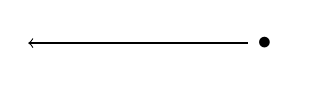
\begin{tikzpicture}
  \draw (0, 0) node (y1) {$\bullet$}; % this can be replaced
  \draw [->] (y1) to ($(y1)-(3, 0)$); % this can not be replaced
\end{tikzpicture}

\end{document}

